

\documentclass{beamer}
 
\usepackage[utf8]{inputenc}
 \usetheme{Madrid}
 \usecolortheme{beaver}
 \usefonttheme{structuresmallcapsserif}
 \usepackage{listings}
%Information to be included in the title page:


\title[Distributed Systems] %optional
{Introduction to Distributed systems}

\subtitle{An Overview}

\author[Dr. Joseph Kehoe] % (optional, for multiple authors)
{Joseph Kehoe\inst{1}}

\institute[IT Carlow] % (optional)
{
	\inst{1}%
	Department of Computing and Networking\\
	Institute of Technology Carlow
}

\date[ITC 2018] % (optional)
{CDD101, 2018}

\logo{
\includegraphics[height=1.5cm]{../../itcarlowlogo.png}}




 
 \AtBeginSection[]
 {
 	\begin{frame}
 		\frametitle{Table of Contents}
 		\tableofcontents[currentsection]
 	\end{frame}
 }
 
 
 
\begin{document}
 
\frame{\titlepage}
 
 
 


  \begin{frame}
  	\frametitle{Definition}
  	\begin{description}
  		\item[Distributed System] A distributed system is a collection of independent computers that appears to its users as a single coherent system
  	\end{description}
\begin{itemize}
	\item   	Distributed systems becomming more common every year. 
  	\item It is important to understand the constraints surrounding the development and usage of distributed systems
\end{itemize}
  	
  		%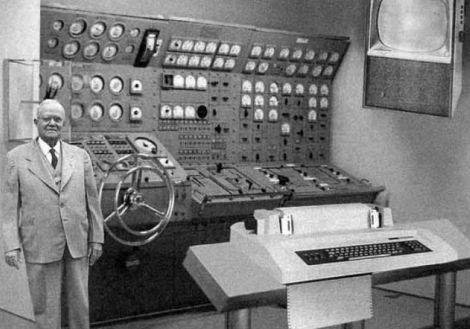
\includegraphics[height=4cm]{Old-Server.jpg}
  \end{frame}
  \begin{frame}
  	\frametitle{Why use them?}
  	\begin{itemize}
  		\item They allow us to connect users and resources
  		\item Data Sharing
  		\item Supercomputing
  		\item Scalabiltiy
  	\end{itemize}
  \end{frame}
  \begin{frame}
  	\frametitle{The Web}
  	\begin{itemize}
  		\item The largest distributed system in the world
  		\item Allows data sharing and compute cycle sharing
  		\item Built on ubiquitous middleware libraries (http, cgi, etc.)
  		\item Open and Transparent
  	\end{itemize}
  \end{frame}
    \begin{frame}
    	\frametitle{Supercomputers}
    	\begin{itemize}
    		\item Almost every entry in top 500 supercomputer list uses "off the shelf" hardware
    		\item Relies on running software over clusters of 100,000's CPUs
    		\item Each CPU has its own memory and distributes load (compute cycles and data) over entire cluster
    	\end{itemize}
    \end{frame}
  \begin{frame}
  	\frametitle{Issues}
  	All the problems of concurrency plus...
  	\begin{itemize}
  		\item Security
  		\item Synchronisation
  		\item Reliability
  		\item Fault Tolerence
  		\item Replication
  		\item Communication
  		\item Scalability
  		\item Naming
  		\item Sharing
  	\end{itemize}
  \end{frame}
    \begin{frame}
    	\frametitle{Hardware}
    	\begin{itemize}
    		\item Multicore and manycore (Xeon Phi)
    		\item GPU (Nvidea)
    		\item Custom Clusters (Supercomputers)
    		\item Homogeneous multicomputers (see above)
    		\item Heterogeneous Computer Systems (Web, Cloud)
    	\end{itemize}
    \end{frame}
      \begin{frame}
      	\frametitle{Software}
      	\begin{itemize}
      		\item Distributed Operating System (many attempts)
      		\item Network Operating System (Unix?)
      		\item Middleware (Http, MPI, Corba, RMI, etc.)
      	\end{itemize}
      \end{frame}
\end{document}

